\subsection{Sprint 4: da 2024-05-22 a 2024-06-03}
\par A seguito del raffinamento della ricerca semantica e di una prima integrazione tra
front-end e back-end, assieme alla definizione di quattro macrocategorie di metriche
di qualità, il gruppo ha optato per la selezione degli strumenti e tecnologie definitive per affrontare lo sviluppo del \glossario{Proof of Concept}.
Si è inoltre concordata la necessità di un ambiente di sviluppo condiviso per limitare i conflitti dipendenti da configurazioni differenti nelle macchine locali. Infine, il gruppo ha ritenuto opportuna una selezione delle \glossario{metriche} individuate in base alla loro predisposizione al calcolo automatico, con conseguente ricerca di strumenti che lo attuino.

\subsubsection{Obiettivi}
\begin{itemize}
  \item Stesura dei verbali interni ed esterni;
  \item Aggiornamento del \PdP\ con conclusione della stesura del consuntivo dello sprint precedente;
  \item Creazione e connessione al database;
  \item Sviluppo e test di un modulo di login per il profilo Tecnico;
  \item \glossario{Dockerizzazione} dell'ambiente di sviluppo;
  \item Caricamento del dizionario dati e test di correttezza per la struttura JSON;
  \item Scelta definitiva del/dei \glossario{LLM} da adottare;
  \item Configurazione di un ambiente per i test di unità;
  \item Sviluppo della funzionalità di debug e visualizzazione del processo di generazione del \glossario{prompt};
  \item Individuazione delle metriche più significative e di strumenti per automatizzarne il calcolo;
  \item Aggiornamento dei documenti \NdP, \Gls\ e \AdR;
\end{itemize}

\begin{figure}[H]
  \centering
  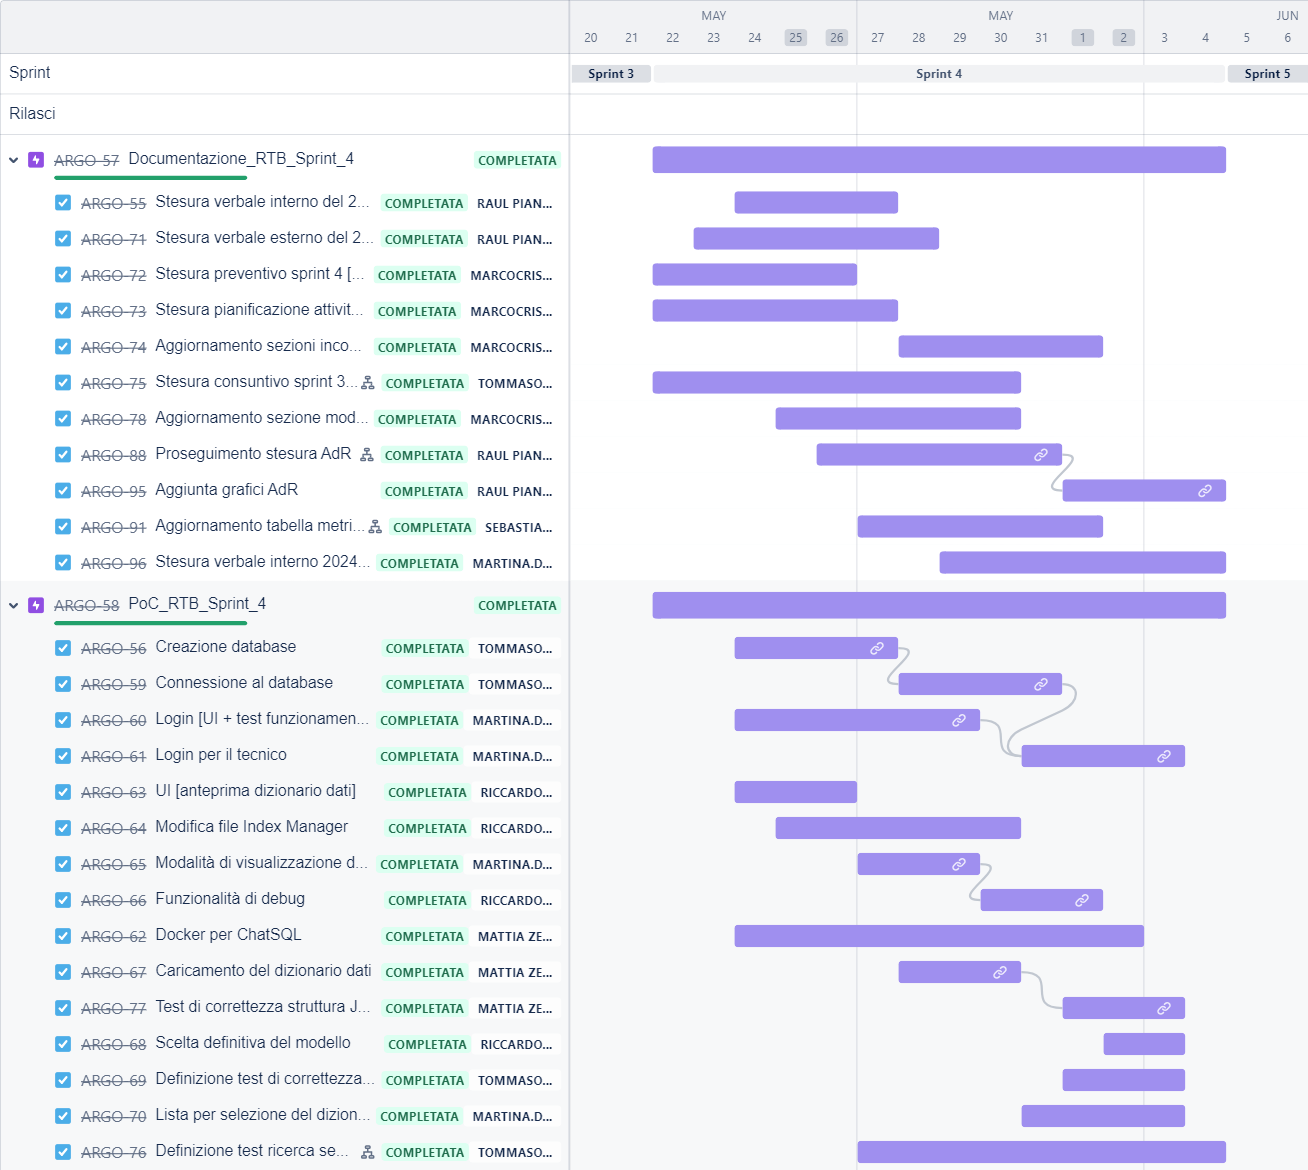
\includegraphics[width=0.90\textwidth]{assets/Pianificazione/Sprint-4/gantt.png}
  \caption{Sprint 4 - Diagramma di Gantt}\label{fig:sprint-4-gantt}
\end{figure}